\clearpage
\subsection{Task 5: การเฝ้าระวังความปลอดภัยบัญชีผู้เล่น (Account Security Monitoring)}
\label{subsec:task5}

% ----------------------------------------------------------------------
% Part 1: บริบททางธุรกิจและกลไกของ Metric F3
% ----------------------------------------------------------------------
\subsubsection{บริบททางธุรกิจและกลไกของตัวชี้วัด \texorpdfstring{$F_3$}{F3}}
\label{subsubsec:t5_business_f3}

ภารกิจที่ 5 มุ่งเน้นการตรวจจับบัญชีผู้เล่นที่มีพฤติกรรมผิดปกติหรือเป็นภัยคุกคามทางความปลอดภัยของระบบเกมออนไลน์ (Account Security Monitoring) สำหรับบริษัท Karena Thailand ซึ่งเผชิญปัญหาบัญชีถูกโจรกรรมที่ยืนยันผลแล้วมากกว่า 5,000 บัญชีต่อเดือน (และคาดว่าตัวเลขจริงสูงกว่า 2 เท่า) ส่งผลให้กลายเป็นปัญหาอันดับหนึ่งของฝ่ายบริการลูกค้า โดยต้องสูญเสียทรัพยากรของทีมสนับสนุนถึง 60\% ของภาระงานทั้งหมด นอกจากนี้ระบบนิเวศของเกมยังถูกคุกคามจากขบวนการซื้อขายบัญชี (Account Selling Rings) ที่ทำลายความสมดุลของการแข่งขัน ฟาร์มบอทที่ทำงานต่อเนื่องตลอด 24 ชั่วโมงจนเกิดภาวะเงินเฟ้อในระบบเศรษฐกิจเกม รวมถึงผู้เล่นที่ใช้ VPN เพื่อปลอมแปลงภูมิภาคและใช้สิทธิ์ราคาส่วนลดข้ามภูมิภาคสูงถึง 70\% ซึ่งสร้างความเสียหายคิดเป็นมูลค่าหลายล้านบาทต่อปี

ระบบรักษาความปลอดภัยแบบกฎตายตัว (Rigid Rule-Based System) ที่ใช้งานอยู่เดิมมีอัตราการแจ้งเตือนผิดพลาด (False Positive Rate) สูงถึง 60\% ตัวอย่างเช่น การล็อกบัญชีนักเดินทางที่ล็อกอินจากต่างประเทศอย่างถูกต้องตามกฎหมาย หรือผู้เล่นที่ฝึกฝนจนทักษะพัฒนาขึ้นอย่างรวดเร็ว ในขณะที่กลับตรวจไม่พบผู้โจมตีที่ชาญฉลาดซึ่งเว้นระยะเวลา 24 ชั่วโมงระหว่างการกระทำ หรือฟาร์มบอทที่มีพฤติกรรมสม่ำเสมอตลอดเวลา ด้วยเหตุนี้ ภารกิจนี้จึงออกแบบเป็นปัญหาการตรวจจับความผิดปกติแบบไม่มีผู้สอน (Unsupervised Anomaly Detection) บนชุดข้อมูลทดสอบเพียงอย่างเดียวจำนวน 25,889 บัญชี โดยไม่มีป้ายกำกับเฉลย (\feat{is\_anomaly}) สำหรับฝึกสอนโมเดล

เกณฑ์การประเมินผลของ Task 5 คือคะแนน $F_3$ ของคลาสผิดปกติ (Anomaly Class) ซึ่งกำหนดค่า $\beta = 3$ ในสมการ $F_\beta$ ดังนี้
\begin{equation}
F_3 = \frac{(1 + 3^2) \cdot \text{Precision} \cdot \text{Recall}}{3^2 \cdot \text{Precision} + \text{Recall}} = \frac{10\,TP}{10\,TP + 9\,FN + FP} = \frac{10\,TP}{9P + \hat{P}}
\label{eq:t5_f3}
\end{equation}
โดยที่ $P = TP + FN$ คือจำนวนบัญชีผิดปกติทั้งหมดที่แท้จริง และ $\hat{P} = TP + FP$ คือจำนวนบัญชีทั้งหมดที่ระบบตัดสินใจแจ้งเตือน สมการ~(\ref{eq:t5_f3}) แสดงให้เห็นว่าค่าน้ำหนักของการพลาดตรวจจับ ($FN$) สูงกว่าค่าปรับจากการแจ้งเตือนผิดพลาด ($FP$) ถึง $\beta^2 = 9$ เท่า

หากพิจารณานโยบายการคัดเลือกบัญชีเพิ่มเข้าสู่ชุดแจ้งเตือนอีก 1 บัญชีที่มีความน่าจะเป็นที่จะผิดปกติจริงเท่ากับ $p$ ค่าคาดหวังของตัวเศษจะเพิ่มขึ้น $10p$ ขณะที่ตัวส่วน $9P + \hat{P}$ จะเพิ่มขึ้นเพียง 1 (เนื่องจาก $P$ คงที่) ดังนั้นการเพิ่มบัญชีดังกล่าวจะช่วยยกระดับค่าคาดหวังของ $F_3$ ก็ต่อเมื่อ
\begin{equation}
\frac{10(TP + p)}{9P + \hat{P} + 1} > \frac{10\,TP}{9P + \hat{P}} \iff p > \frac{TP}{9P + \hat{P}} = \frac{F_3}{1 + \beta^2} = \frac{F_3}{10}
\label{eq:t5_breakeven}
\end{equation}
ภายใต้ระดับประสิทธิภาพเป้าหมาย $F_3 \in [0.80, 1.00]$ จุดคุ้มทุนของความน่าจะเป็นในการคัดเลือกบัญชีเข้าสู่ชุดแจ้งเตือน ($p^*$) จะอยู่ที่เพียงประมาณ 8\textendash 10\% เท่านั้น (เช่น ที่ $F_3 \approx 0.997$ จุดคุ้มทุนคือ $p^* \approx 9.97\%$) คุณสมบัติทางคณิตศาสตร์นี้บังคับให้การออกแบบระบบต้องไม่พลาดกลุ่มผิดปกติขนาดย่อมใดๆ ขณะเดียวกันก็ต้องหลีกเลี่ยงการปนเปื้อนบัญชีปกติที่มีความน่าจะเป็นต่ำกว่า 8\% เข้ามาในผลลัพธ์

% ----------------------------------------------------------------------
% Part 2: ข้อค้นพบจาก EDA และโครงสร้างการสร้างข้อมูล
% ----------------------------------------------------------------------
\subsubsection{ข้อค้นพบจาก EDA และโครงสร้างการสร้างข้อมูล}
\label{subsubsec:t5_eda}

\begin{insightbox}[ข้อค้นพบสำคัญ: ความเป็นอิสระของฟีเจอร์ปกติและวงจรสกัดความผิดปกติจากส่วนเหลือ (Residual Discovery Loop)]
\begin{itemize}
  \item \textbf{ข้อสมมติฐาน (Claim):} บัญชีผู้เล่นปกติถูกสร้างขึ้นจากฟีเจอร์เชิงพฤติกรรมที่มีความเป็นอิสระต่อกันเกือบสมบูรณ์ (Near-Independent Marginals) ในขณะที่ความผิดปกติแต่ละประเภทไม่ใช่หางการแจกแจงแบบต่อเนื่อง (Smooth Tail) แต่เป็นกลุ่มที่ถูกฉีดแทรกด้วยกลไกชัดเจนซึ่งทำลายความเป็นอิสระดังกล่าวใน 3 รูปแบบ ได้แก่ การกระชากข้ามเวลา กลุ่มแยกบนฮิสโทแกรม 1 มิติ และกล่องความแปรปรวนร่วมในหลายมิติ
  \item \textbf{หลักฐานเชิงประจักษ์ (Evidence):} บนชุดข้อมูลทดสอบ v2 ($N = 25{,}889$) ค่าสหสัมพันธ์เชิงเส้นระหว่างค่าเฉลี่ย 4 ช่วงเวลาของฟีเจอร์ต่อเนื่องและฟีเจอร์สถิติทุกคู่มีค่ามัธยฐาน $|r| = 0.0049$ และสูงสุด $|r| = 0.2403$ แต่เมื่อถอดบัญชีผิดปกติทั้ง 2,104 บัญชีที่ตรวจพบออกแล้ว กลุ่มบัญชีปกติส่วนเหลือ (23,785 บัญชี) มีค่ามัธยฐาน $|r| = 0.0044$ และค่าสูงสุด $|r|$ ลดลงเหลือเพียง $0.0263$
  \item \textbf{นัยเชิงวิศวกรรม (Implication):} แทนที่จะจัดอันดับด้วยคะแนนความผิดปกติแบบกล่องดำ (Black-Box Anomaly Score) ซึ่งไม่สามารถกำหนดจุดตัดได้โดยไม่มี Label เราสามารถออกแบบ \textbf{วงจรสกัดความผิดปกติจากส่วนเหลืออย่างเป็นระบบ (Systematic Residual Discovery Loop)} ที่ค้นพบกลุ่มผิดปกติทีละชั้น ตัดออก แล้วสแกนส่วนที่เหลือซ้ำจนกระทั่งโครงสร้างส่วนเหลือคืนสู่ระดับสัญญาณรบกวนอิสระ
\end{itemize}
\end{insightbox}

จากการวิเคราะห์ข้อมูลเชิงลึกด้วยวงจรส่วนเหลือบนชุดข้อมูล v2 ($N = 25{,}889$) ระบบสามารถจำแนกโครงสร้างความผิดปกติออกเป็น 4 ชั้น (4-Stage Union) รวมทั้งสิ้น 2,104 บัญชี (8.13\%) โดยไม่มีการซ้อนทับกันระหว่างชั้นเลย (0 overlaps) ดังรายละเอียดต่อไปนี้

\begin{enumerate}
  \item \textbf{Stage A \textemdash\ การกระชากข้ามเวลา (Temporal Shock: 827 บัญชี, 39.3\% ของบัญชีที่แจ้งเตือน):} เมื่อเปรียบเทียบพฤติกรรมในช่วงเวลาที่ 3 และ 4 เทียบกับค่าฐานในช่วงเวลาที่ 1\textendash 2 ของบัญชีเดียวกัน พบกลุ่มประชากรที่แยกตัวออกจากบัญชีปกติอย่างชัดเจนที่เกณฑ์ค่ามาตรฐานแบบแกร่งอันดับที่สอง $z_2 > 6$ จำนวน 816 บัญชี บวกกับบัญชีที่มีการกระโดดของพิกัดล็อกอิน $> 5^\circ$ หรือมีค่าละติจูดผิดวิสัย ($|\text{lat}| > 90$) โดยไม่เข้าเกณฑ์ $z_2 > 6$ อีก 11 บัญชี รวมเป็น 827 บัญชี (รูปที่~\ref{fig:t5_shock_gaps}(a)) กลุ่มนี้แยกออกเป็น 4 ประเภทย่อย ได้แก่ \textbf{Takeover (310)} ที่มีการโอนเงินในเกมและเปลี่ยนอุปกรณ์/ตำแหน่งพุ่งสูงพร้อมความสม่ำเสมอการเล่นตกฮวบ, \textbf{Selling (311)} ที่ค่า \feat{skill\_rating}, \feat{kda\_mean}, \feat{accuracy\_mean} พุ่งขึ้นพร้อมปฏิกิริยาไวขึ้นและการลบเพื่อน, \textbf{VPN (198)} ที่ยอดและความถี่การซื้อเพิ่มฉับพลันร่วมกับการเปลี่ยนตำแหน่ง และ \textbf{Geo-only (8)} ที่มีการย้ายพิกัดล็อกอินอย่างเดียว
  \item \textbf{Stage B \textemdash\ กลุ่มแยก 1 มิติที่มีช่องว่างฮิสโทแกรม (1-D Empty Histogram Gaps: 981 บัญชี, 46.6\%):} การสแกนฮิสโทแกรม 80 ช่วง (80-bin Histogram) บนบัญชีที่อยู่นอก Stage A เผยให้เห็นกลุ่มก้อนขนาดกะทัดรัด 4 กลุ่มที่ถูกคั่นออกจากบัญชีปกติด้วยช่องว่างสนิท ($\ge 3$ ช่องติดต่อกันที่มีความหนาแน่น $\le 2\%$ ของค่าฐาน; รูปที่~\ref{fig:t5_shock_gaps}(b)\textendash (e)) ได้แก่
    \begin{itemize}
      \item \textbf{Low Activity (265):} ค่าเฉลี่ย 4 ช่วงเวลาของ \feat{activity\_level} $< 0.345$ โดยมีช่องว่างสนิทในช่วง $[0.27, 0.41]$
      \item \textbf{Low Communication (263):} ค่าเฉลี่ย 4 ช่วงเวลาของ \feat{communication\_frequency} $< 0.169$ โดยมีช่องว่างสนิทในช่วง $[0.09, 0.24]$
      \item \textbf{Low Stability (246):} ฟีเจอร์คงที่ \feat{behavior\_stability} $< 0.473$ ซึ่งถูกคั่นด้วยช่องว่างขนาดกว้าง $[0.40, 0.70]$ โดยไม่มีบัญชีใดอยู่ระหว่างกลางเลย
      \item \textbf{Bot (207):} ปรากฏเป็นกลุ่มบัญชีชุดเดียวกันเป๊ะ (207/207) ใน 4 ฟีเจอร์พร้อมกัน ได้แก่ \feat{ip\_hash\_entropy} $< 0.238$ (ช่องว่าง $[0.17, 0.31]$), \feat{kda\_std} $< 0.151$, \feat{login\_time\_variance} $< 1.082$ และ \feat{session\_duration\_std} $< 6.297$
    \end{itemize}
  \item \textbf{Stage C \textemdash\ กล่องความแปรปรวนร่วม 3 มิติ (Joint 3-D Acc/KDA Box: 244 บัญชี, 11.6\%):} กลุ่มนี้มองไม่เห็นในฮิสโทแกรม 1 มิติเลยเนื่องจากแต่ละฟีเจอร์มีค่ากระจายอยู่ภายในช่วงปกติ แต่เมื่อทำการทดสอบการเกิดร่วมกันของหาง 5\% (Pairwise 5\%-Tail Co-occurrence $z$-test) บนบัญชีส่วนเหลือ 24,081 บัญชี พบคู่ขอบเดียวที่มีนัยสำคัญสูงมาก คือหางบนของ \feat{accuracy\_std} $\times$ หางบนของ \feat{kda\_std} เกิดร่วมกัน 222 ครั้งเทียบกับค่าคาดหวังอิสระ 60.2 ครั้ง ($z = 20.9$) เมื่อต่อยอดด้วยแบบจำลองผสมเกาส์เซียน (2-Component EM) และขยายคุณลักษณะที่มีค่าเฉลี่ยเบี่ยงเบน $> 0.6\,\text{SD}$ พบว่าดึงฟีเจอร์ \feat{performance\_stability} และความผันผวนข้ามช่วงเวลาแบบปรับระดับค่าเฉลี่ย (\feat{performance\_stability\textasciitilde vol}, เบี่ยงเบน $-0.481\,\text{SD}$) เข้ามาร่วมด้วย ขอบเขตของสมาชิกที่มั่นใจ ($\text{posterior} > 0.9$) ก่อตัวเป็นกล่อง 3 มิติรายช่วงเวลาที่คมชัด (รูปที่~\ref{fig:t5_acckda_box}(a)) จับได้ 244 บัญชีด้วยความแม่นยำเทียบฐานการสุ่ม (Null-calibrated Precision) สูงถึง 99.7\%
  \item \textbf{Stage D \textemdash\ สมาชิก Low Stability ที่ถูกซ่อนด้วยค่า NaN (NaN-Hidden LowStab: $+52$ บัญชี, 2.5\%):} เนื่องจากคอลัมน์ \feat{behavior\_stability} มีค่าหายไป (\feat{NaN}) ใน 1,257 บัญชี (4.86\%) จึงมีสมาชิกกลุ่ม \feat{lowstab} ประมาณ 13 บัญชี ($246 \times 0.0486 / (1 - 0.0486) \approx 12.6$) หลุดรอดจากกฎ Stage B3 เมื่อคัดกรองบัญชีที่ \feat{behavior\_stability} เป็น \feat{NaN} นอกชุด A\textendash C แต่มีทุกช่วงเวลาที่สังเกตได้ตกอยู่ในกล่องคุณลักษณะของกลุ่ม \feat{lowstab} (\feat{purchase\_frequency} $\in [3, 6]$ และ \feat{account\_age\_days} $\in [800, 1500]$) พบผู้สมัครนอกชุด A\textendash C ทั้งหมด 128 บัญชี (หรือ 129 บัญชีก่อนหัก 1 แถวที่ซ้อนทับใน Stage C) เทียบกับค่าคาดหวังโดยบังเอิญ 109 บัญชี การคำนวณความน่าจะเป็นภายหลังแบบ Naive Bayes ด้วยฟีเจอร์เสริม 2 ตัวที่จุดตัด $> 0.10$ ช่วยกู้คืนบัญชีเพิ่มเข้ามาได้อีก 52 บัญชี
\end{enumerate}

\begin{figure}[H]
\centering
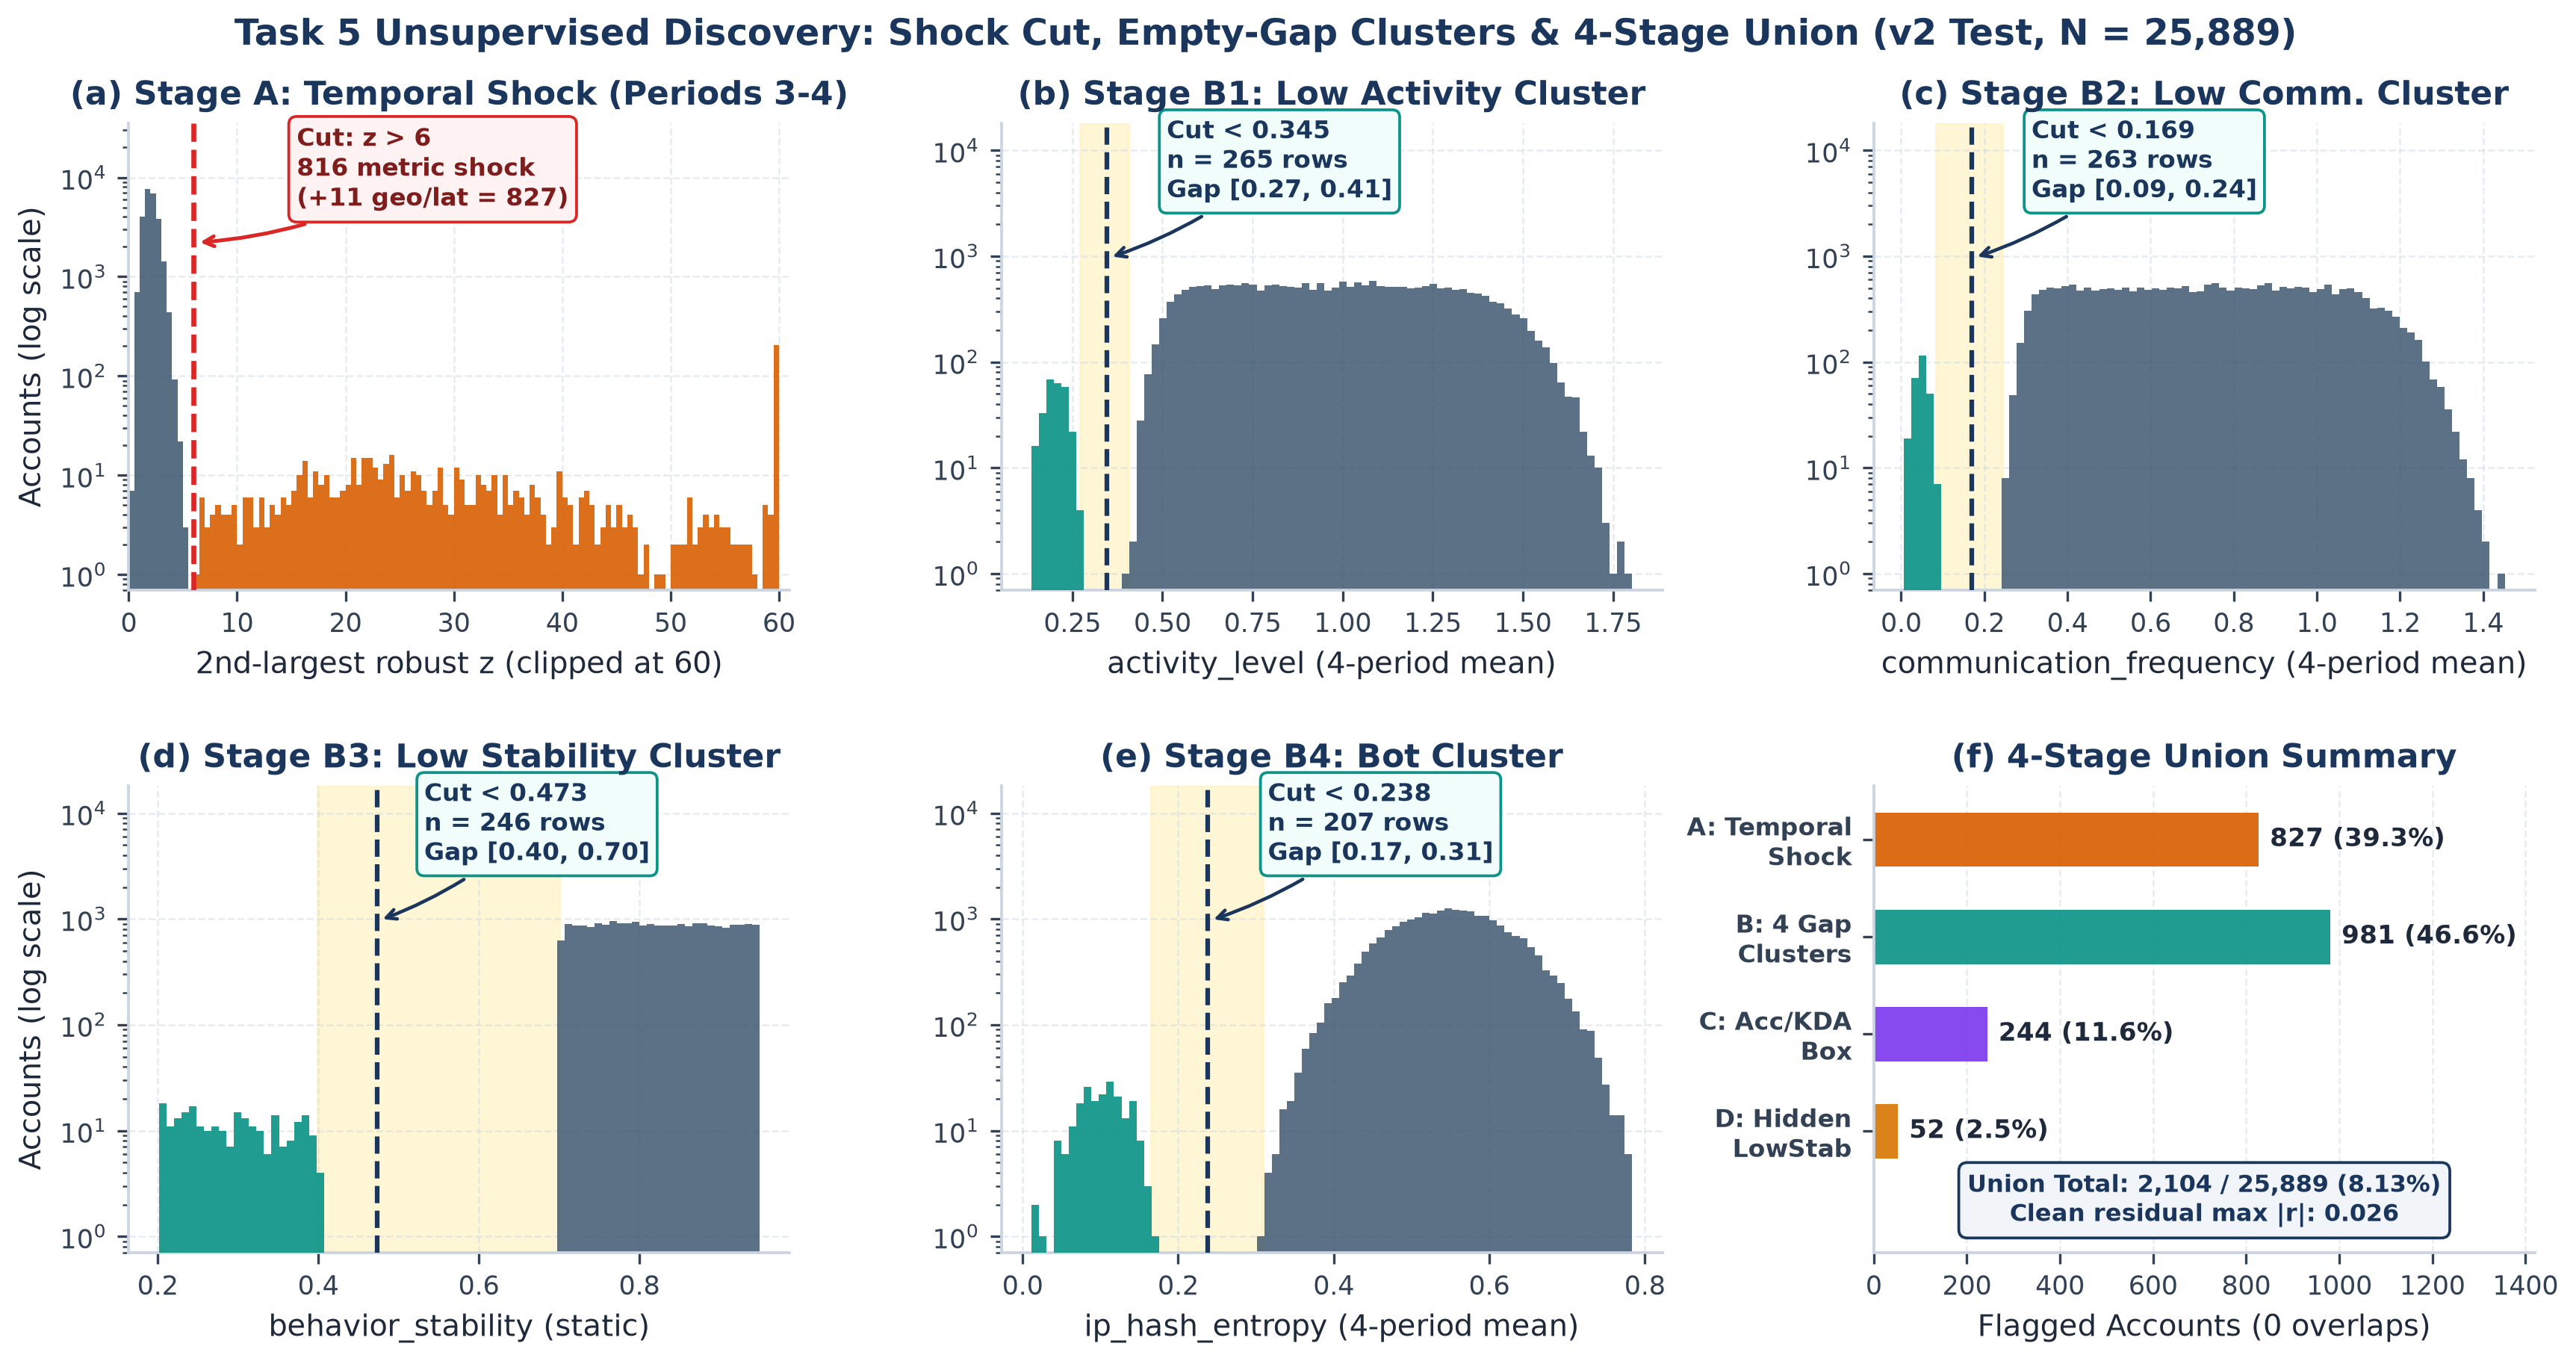
\includegraphics[width=0.98\textwidth]{figures/t5/fig_t5_shock_and_gaps.png}
\caption{ผลการค้นพบความผิดปกติแบบไม่มีผู้สอนบนชุดข้อมูลทดสอบ v2 ($N = 25{,}889$): (a) จุดตัดค่า $z_2 > 6$ ของ Stage A Temporal Shock (816 บัญชีจากความต่างเมตริก $+ 11$ จาก Geo/Lat $= 827$); (b)\textendash (e) กลุ่มแยก 1 มิติใน Stage B ทั้ง 4 กลุ่มที่ถูกคั่นจากบัญชีปกติด้วยช่องว่างฮิสโทแกรมสนิท; และ (f) สรุปสัดส่วนการรวมผล 4 ชั้นรวม 2,104 บัญชี (8.13\%) โดยไม่มีการซ้อนทับและส่วนเหลือสะอาดมี $\max |r| = 0.026$}
\label{fig:t5_shock_gaps}
\end{figure}

\begin{figure}[H]
\centering
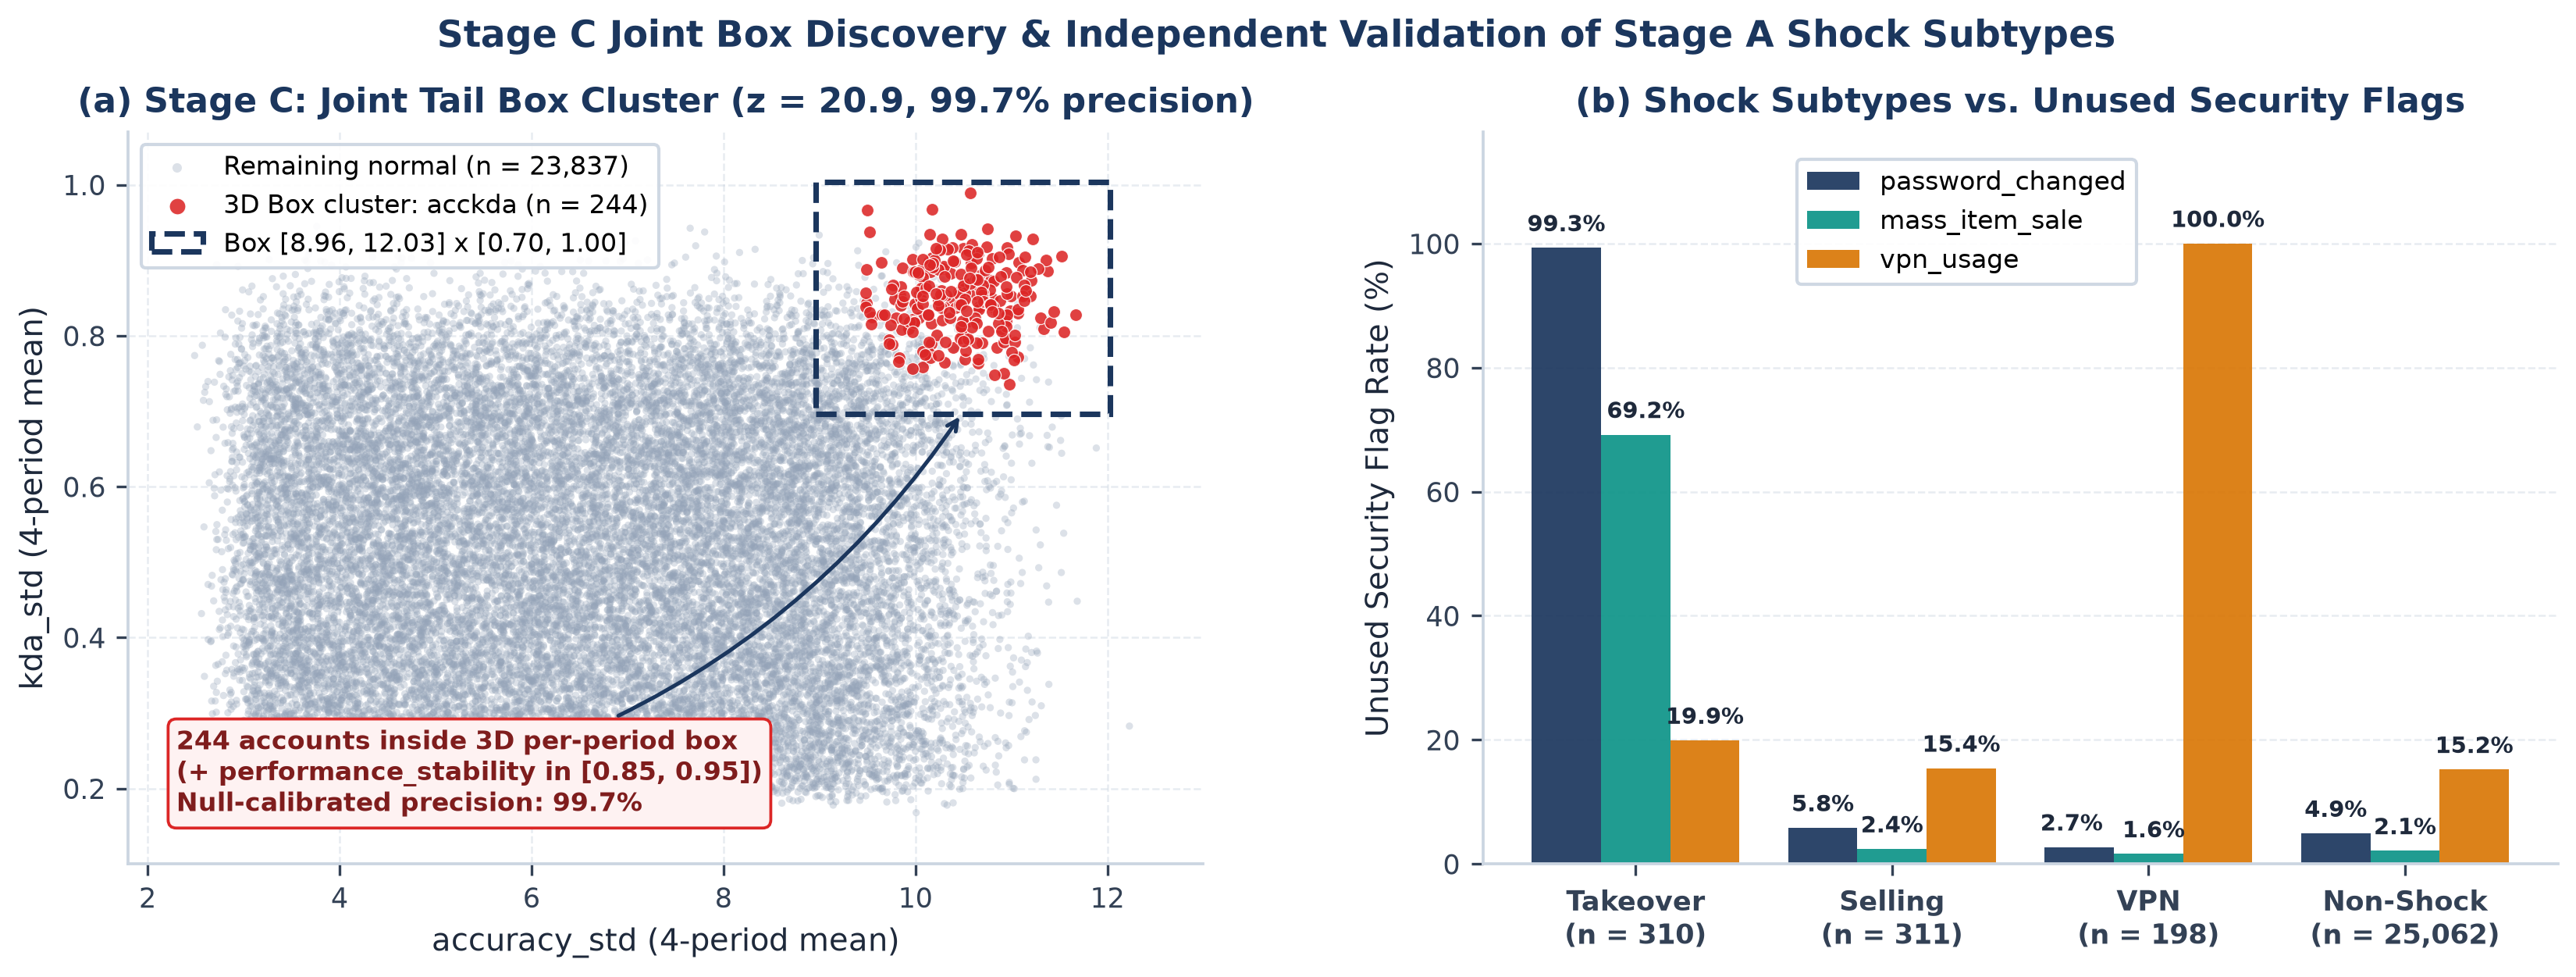
\includegraphics[width=0.98\textwidth]{figures/t5/fig_t5_acckda_box.png}
\caption{(a) การค้นพบกลุ่มกล่อง 3 มิติใน Stage C (\protect\feat{accuracy\_std} $\in [8.96, 12.03]$, \protect\feat{kda\_std} $\in [0.70, 1.00]$ ร่วมกับ \protect\feat{performance\_stability} $\in [0.85, 0.95]$) จากค่าสถิติการเกิดร่วมกัน $z = 20.9$ ได้ 244 บัญชีด้วยความแม่นยำ 99.7\%; และ (b) การตรวจสอบยืนยันแยกส่วน (Independent Validation) ด้วย Security Flags ที่ไม่ได้ถูกนำไปใช้ในกฎการตรวจจับ ซึ่งสอดคล้องกับประเภทย่อยของ Stage A อย่างชัดเจน}
\label{fig:t5_acckda_box}
\end{figure}

% ----------------------------------------------------------------------
% Part 3: การเตรียมข้อมูลและการจัดการค่าที่หาย
% ----------------------------------------------------------------------
\subsubsection{การเตรียมข้อมูลและการจัดการค่าที่หาย}
\label{subsubsec:t5_preprocessing}

ชุดข้อมูล Task 5 มีเฉพาะข้อมูลทดสอบจำนวน 25,889 แถวและ 122 ฟีเจอร์ดิบ (ไม่นับ \feat{player\_id}) ประกอบด้วย 29 เมตริกเชิงเวลาที่วัดซ้ำใน 4 ช่วงเวลาต่อเนื่อง (ต่อท้าย \feat{\_1} ถึง \feat{\_4} รวม 116 คอลัมน์) ร่วมกับ 2 ฟีเจอร์สถิติต่อเนื่อง (\feat{account\_age\_days}, \feat{behavior\_stability}) และ 4 Security Flags แบบไบนารี (\feat{password\_changed}, \feat{vpn\_usage}, \feat{suspicious\_login\_time}, \feat{mass\_item\_sale}) ภาพรวมข้อมูลมีอัตราค่าที่หายไป (\feat{NaN}) เฉลี่ย 4.88\% (ราว 5\%) ทั่วทุกฟีเจอร์ และคอลัมน์ \feat{behavior\_stability} มีค่าหายไป 1,257 บัญชี (4.86\%) ระบบได้กำหนดมาตรฐานการเตรียมข้อมูลและจัดการค่าที่หายไว้ 4 ประการ ดังนี้

\begin{enumerate}
  \item \textbf{การจัดการพิกัดละติจูดผิดวิสัย ($|\text{lat}| > 90$):} พบ 71 บัญชีที่มีค่า \feat{login\_lat\_p} เกินขอบเขตทางกายภาพ $[-90, 90]$ แทนที่จะลบทิ้งหรือเติมค่ามัธยฐานซึ่งจะทำลายหลักฐานการปลอมแปลงพิกัด ระบบบันทึกธง \feat{bad\_lat} เพื่อแจ้งเตือนใน Stage A ทันที แล้วจึงแทนที่ค่าพิกัดที่ผิดปกติเหล่านั้นด้วย \feat{NaN} ก่อนคำนวณจุดศูนย์กลางฐานบ้าน $(\bar{\phi}_{1:2}, \bar{\lambda}_{1:2})$ และการคำนวณระยะห่างเชิงมุมข้ามเส้นแบ่งเขตวันด้วยสูตรห่อหุ้มลองจิจูด $((\lambda - \bar{\lambda}_{1:2} + 180) \bmod 360) - 180$
  \item \textbf{ฐานเวลาและการปรับสเกลแบบแกร่ง (NaN-Safe Robust Statistics):} ค่าฐานช่วง 1\textendash 2 คำนวณด้วย \feat{nanmean} และความเปลี่ยนแปลงในช่วง 3\textendash 4 คำนวณด้วย $\max_{p \in \{3,4\}} |x_p - \bar{x}_{1:2}|$ จากนั้นแปลงเป็น Robust $z$-score เทียบกับค่ามัธยฐานและ $\text{MAD}$ ($1.4826 \cdot \text{median}(|\Delta - \text{med}|)$) ของประชากรทั้งหมด ค่า $z$ ที่ขาดหายถูกกำหนดให้เป็น 0 หลังการปรับสเกลเพื่อป้องกันการแจ้งเตือนเท็จจากค่าว่าง ร่วมกับเงื่อนไขที่กำหนดให้ค่า $z$ อันดับที่ 2 ($z_2$) ต้องเกิน 6 เพื่อกรองสัญญาณรบกวนที่เกิดกับฟีเจอร์เดียว
  \item \textbf{การคงค่า \feat{NaN} ไว้ภายในการตรวจสอบกล่อง \feat{allin()}:} เนื่องจากระบบตัวสร้างข้อมูลฉีดความผิดปกติแบบคงที่ (Stationary Types) ด้วยการสุ่มสม่ำเสมอรายช่วงเวลาภายในกล่องขอบเขตปิด แต่ข้อมูลยังคงมีค่าหายสุ่มราว 5\% ต่อช่วงเวลา หากใช้การเติมค่าเฉลี่ยหรือมัธยฐานก่อนตรวจสอบขอบเขต บัญชีผิดปกติที่มีค่าหายเพียง 1 ช่วงเวลา (ซึ่งคิดเป็นโอกาสถึง $1 - 0.95^4 \approx 18.5\%$ ของบัญชีทั้งหมด) จะถูกดึงออกนอกกล่องทันที ระบบจึงออกแบบเงื่อนไขการตรวจกล่องทุกชนิดด้วยตัวดำเนินการ \feat{((m >= lo) \& (m <= hi)) | isnan(m)} ครบทั้ง 4 ช่วงเวลา เพื่อให้ค่าที่สังเกตได้จริงทั้งหมดเป็นตัวตัดสินโดยไม่สูญเสียความครอบคลุม
  \item \textbf{การคำนวณ Naive Bayes Likelihood Ratio แบบรองรับค่า \feat{NaN}:} สำหรับผู้สมัครที่ \feat{behavior\_stability} เป็น \feat{NaN} แต่ตกอยู่ในกล่องเสริม \feat{purchase\_frequency} $\in [3, 6]$ และ \feat{account\_age\_days} $\in [800, 1500]$ ระบบคำนวณ Log-Likelihood Ratio (LLR) จากฮิสโทแกรมปรับเรียบ (Laplace Smoothing $\alpha = 0.5$) ของฟีเจอร์ 2 ตัว โดยให้พจน์ของฟีเจอร์ที่มีค่า \feat{NaN} มีค่า $\text{LLR} = 0$ (Marginalization) เพื่อป้องกันอคติจากการเติมค่าเทียม
\end{enumerate}

% ----------------------------------------------------------------------
% Part 4: การออกแบบระบบตรวจจับและเหตุผลเชิงวิศวกรรม
% ----------------------------------------------------------------------
\subsubsection{การออกแบบระบบตรวจจับและเหตุผลเชิงวิศวกรรม}
\label{subsubsec:t5_architecture}

สถาปัตยกรรมตรวจจับสุดท้าย (\feat{t5v2\_union\_box\_lsnan.csv}) เป็นการผสานแบบ Hard-OR Union ของตัวตรวจจับทางสถิติและตัวแบบความน่าจะเป็นเชิงตีความได้จำนวน 4 ชั้น บนชุดข้อมูลทดสอบ 25,889 บัญชี โดยมีโครงสร้างสรุปดังตารางที่~\ref{tab:t5_detectors}

\begin{table}[htbp]
\centering
\caption{สถาปัตยกรรมตัวตรวจจับแบบ 4 ชั้น (4-Stage Union) และกลุ่มย่อยความผิดปกติทั้ง 8 ประเภทบนชุดข้อมูล v2 ($N = 25{,}889$)}
\label{tab:t5_detectors}
\small
\begin{tabular}{@{} >{\raggedright\arraybackslash}p{2.3cm} >{\raggedright\arraybackslash}p{2.6cm} >{\raggedright\arraybackslash}p{5.8cm} r r @{}}
\toprule
\textbf{ชั้น (Stage)} & \textbf{กลุ่ม / ประเภทย่อย} & \textbf{เกณฑ์ตรวจจับและขอบเขต (Rule / Box)} & \textbf{จำนวน} & \textbf{สัดส่วน (\%)} \\
\midrule
\multirow{4}{=}{A: Temporal Shock (827 บัญชี)}
 & Takeover & $z_2 > 6$ (ช่วง 3\textendash 4 เทียบ 1\textendash 2); โอนเงิน/เปลี่ยนตำแหน่ง/อุปกรณ์พุ่ง, \feat{play\_pattern\_consistency} ตก & 310 & 14.7\% \\
 & Selling & $z_2 > 6$; \feat{skill\_rating}, \feat{kda\_mean}, \feat{accuracy\_mean} พุ่ง, ลบเพื่อนเพิ่ม & 311 & 14.8\% \\
 & VPN & $z_2 > 6$; ยอด/ความถี่การซื้อพุ่งร่วมกับตำแหน่งเปลี่ยน & 198 & 9.4\% \\
 & Geo-only & ย้ายพิกัด $> 5^\circ$ หรือ $|\text{lat}| > 90$ โดย $z_2 \le 6$ & 8 & 0.4\% \\
\midrule
\multirow{4}{=}{B: 1-D Empty Gaps (981 บัญชี)}
 & Bot & ค่าเฉลี่ย 4 ช่วง: \feat{ip\_hash\_entropy} $< 0.238$, \feat{kda\_std} $< 0.151$, \feat{login\_time\_variance} $< 1.082$, \feat{session\_duration\_std} $< 6.297$ & 207 & 9.8\% \\
 & Low Activity & ค่าเฉลี่ย 4 ช่วง: \feat{activity\_level} $< 0.345$ (ช่องว่าง $[0.27, 0.41]$) & 265 & 12.6\% \\
 & Low Comm. & ค่าเฉลี่ย 4 ช่วง: \feat{communication\_frequency} $< 0.169$ (ช่องว่าง $[0.09, 0.24]$) & 263 & 12.5\% \\
 & Low Stability & ฟีเจอร์สถิติ: \feat{behavior\_stability} $< 0.473$ (ช่องว่าง $[0.40, 0.70]$) & 246 & 11.7\% \\
\midrule
C: Joint 3-D Box & Acc/KDA Box & ทุกช่วงสังเกตใน \feat{accuracy\_std} $[8.96, 12.03]$, \feat{kda\_std} $[0.70, 1.00]$, \feat{performance\_stability} $[0.85, 0.95]$ & 244 & 11.6\% \\
\midrule
D: Hidden LowStab & NaN-Aware NB & \feat{behavior\_stability} เป็น \feat{NaN}, อยู่ใน \feat{purchase\_frequency} $[3,6]$ $\times$ \feat{account\_age\_days} $[800,1500]$, $\text{posterior} > 0.10$ & 52 & 2.5\% \\
\midrule
\multicolumn{3}{@{}l}{\textbf{รวมทั้งหมด (4-Stage Hard-OR Union, 0 Overlaps)}} & \textbf{2,104} & \textbf{100.0\%} \\
\multicolumn{3}{@{}l}{\textit{สัดส่วนการแจ้งเตือนรวมจากบัญชีทั้งหมด (2,104 / 25,889)}} & \multicolumn{2}{r}{\textit{8.13\%}} \\
\bottomrule
\end{tabular}
\end{table}

ใน Stage C ตัวแบบค้นพบกล่อง 3 มิติแบบไร้ผู้สอนโดยอัตโนมัติจากขั้นตอน: (1) สร้างกราฟความสัมพันธ์ของขอบหาง 5\% ที่มี $z > 6$ พบคู่ \feat{accuracy\_std} $\times$ \feat{kda\_std} ($z = 20.9$), (2) ประมาณค่า EM 2-Component (กลุ่มเกาส์เซียนเทียบกับผลคูณความหนาแน่น 1 มิติอิสระของพื้นหลัง) แล้วขยายคุณลักษณะที่มี $| \text{shift} | > 0.6\,\text{SD}$ ซึ่งดึง \feat{performance\_stability} และ \feat{performance\_stability\textasciitilde vol} เข้าร่วมโดยอัตโนมัติ และ (3) ประมาณขอบกล่องรายช่วงเวลาจากสมาชิกที่มี $\text{posterior} > 0.9$ (ควอนไทล์ $0.5\%/99.5\%$ ขยายขอบ 2\%) ซึ่งจะได้ขอบเขต \feat{accuracy\_std} $\in [8.9588, 12.0298]$, \feat{kda\_std} $\in [0.6962, 1.0042]$ และ \feat{performance\_stability} $\in [0.8486, 0.9514]$

สำหรับ Stage D ในกลุ่มผู้สมัคร 129 บัญชีที่เข้าเงื่อนไขกล่องเสริม (หรือ 128 บัญชีเมื่อหัก 1 บัญชีที่อยู่ใน Stage C แล้ว) ค่าสถิติชี้ว่าสมาชิก \feat{lowstab} ที่สังเกตเห็นได้มีค่ามัธยฐาน \feat{login\_count} ต่ำกว่ากลุ่มปกติในกล่องเดียวกันเกือบครึ่ง (34.1 เทียบกับ 58.6) และมีความแปรปรวนรายช่วงเวลาของ \feat{purchase\_frequency} สูงกว่า (0.83 เทียบกับ 0.67) การรวม LLR ของสองคุณลักษณะนี้ร่วมกับค่า Prior $14 / 129 \approx 10.9\%$ และจุดตัด $\text{posterior} > 0.10$ (สอดคล้องกับจุดคุ้มทุนของ $F_3$ ที่ $p^* \approx 10\%$) คัดเลือกได้ 53 บัญชีซึ่งเป็นบัญชีใหม่ที่อยู่นอก Stage A\textendash C จำนวน 52 บัญชี (ค่าคาดหวังความผิดปกติจริงใน 52 บัญชีนี้เท่ากับ 12.4 บัญชี)

\begin{decisionbox}[เหตุผลเชิงวิศวกรรม: เหตุใดตัวตรวจจับเชิงสถิติและ Support Box จึงเหนือกว่าโมเดลกล่องดำ]
\begin{enumerate}
  \item \textbf{ไร้ป้ายกำกับสำหรับตั้งจุดตัด (No Labels for Thresholding):} โมเดลตรวจจับความผิดปกติทั่วไป (เช่น Isolation Forest หรือ Autoencoder) ให้ผลลัพธ์เป็นคะแนนจัดอันดับต่อเนื่อง เมื่อไม่มีป้ายกำกับเฉลยใน Task 5 การเลือกเปอร์เซ็นไทล์จุดตัดจึงกลายเป็นการเดาสุ่ม ตรงกันข้ามกับตัวตรวจจับ 4 ชั้นที่อาศัยช่องว่างสนิทบนฮิสโทแกรม ขอบเขต Robust $z$, กรอบกล่องรายช่วงเวลา และจุดคุ้มทุนทางคณิตศาสตร์ของ $F_3$
  \item \textbf{ขอบเขตของกล่องคมชัดกว่าหางเกาส์เซียน (Hard Box Edges vs.\ Gaussian Smearing):} กลไกการสร้างข้อมูลฉีดกลุ่มคงที่ด้วยค่าสุ่มสม่ำเสมอภายในขอบเขตสี่เหลี่ยมที่คมชัด (เช่น ไม่มีบัญชีใดมี \feat{behavior\_stability} ใน $[0.40, 0.70]$ และบนข้อมูล v1 การบีบขอบกล่อง \feat{acckda} ลง 10\% ทำให้สมาชิกหายไปถึง 73\textendash 92 บัญชี ขณะที่การขยายขอบขึ้น 10\% เพิ่มขึ้นเพียง 0\textendash 1 บัญชี) การใช้จุดตัดความน่าจะเป็นจาก EM (\feat{p50}) บนข้อมูล v1 พลาดบัญชีในกล่องจริงไป 22 แถวและรับผลบวกลวงเข้ามา 12 แถว ขณะที่กฎกล่องรายช่วงเวลามีความแม่นยำสูงถึง 99.7\%
  \item \textbf{ความบอดของโมเดลความหนาแน่นและ Reconstruction ต่อฟีเจอร์ 1\textendash 3 มิติ:} โมเดลมิติสูง (เช่น TMAE, OCSVM, Mahalanobis, PCA) คำนวณระยะทางหรือความคลาดเคลื่อนเฉลี่ยข้ามทุกฟีเจอร์พร้อมกัน ทำให้สัญญาณของกลุ่ม \feat{lowact}, \feat{lowcomm} และ \feat{acckda} ซึ่งมีความผิดปกติเพียง 1\textendash 3 ฟีเจอร์และมีค่าอยู่ภายในขอบเขตปกติ (Marginal Range) ถูกกลบด้วยความแปรปรวนอิสระของอีกกว่า 20 ฟีเจอร์ที่เหลือ ส่วนกลุ่ม \feat{bot} ที่มี 207 บัญชีเกาะกลุ่มแน่นหนาก็หลอกให้ตัววัดความหนาแน่นเชิงพื้นที่อย่าง LOF มองว่าเป็นย่านปกติที่มีความหนาแน่นสูง
\end{enumerate}
\end{decisionbox}

% ----------------------------------------------------------------------
% Part 5: การตรวจสอบความสมบูรณ์และการประเมินผลโดยไม่มี Label
% ----------------------------------------------------------------------
\subsubsection{การตรวจสอบความสมบูรณ์และการประเมินผลโดยไม่มี Label (Validation Without Labels)}
\label{subsubsec:t5_validation}

เนื่องจาก Task 5 ไม่มีป้ายกำกับสำหรับการทำ Cross-Validation แบบมีผู้สอน ทีมจึงออกแบบระบบการตรวจสอบความถูกต้องโดยปราศจาก Label ออกเป็น 4 เสาหลัก ได้แก่

\textbf{1) การพิสูจน์ความสมบูรณ์ของส่วนเหลือ (Residual Completeness Scans):}
หลังจากตัดกลุ่ม 2,104 บัญชีออกแล้ว ค่าสหสัมพันธ์สูงสุดระหว่างฟีเจอร์ในกลุ่มสะอาด 23,785 บัญชีลดเหลือเพียง $\max |r| = 0.0263$ (มัธยฐาน $0.0044$) นอกจากนี้ การสแกนเชิงสถิติระดับต่ำเพื่อค้นหากลุ่มผิดปกติที่อาจซ่อนอยู่เพิ่มเติมให้ผลเป็นระดับ Null ทั้งหมด:
\begin{itemize}
  \item \textbf{Box-Pair Scan (1,040,403 คู่ช่วง):} ในการตรวจสอบโครงสร้างเชิงลึก (v1) การทดสอบทุกคู่ช่วงเวลาข้ามฟีเจอร์จากตัวบ่งชี้กล่อง 1,443 ช่วงสามารถตรวจจับกลุ่ม \feat{bot} ได้ที่ระดับ $z = 126.0$ (207 เทียบกับค่าคาดหวัง 1.7) แต่เมื่อสแกนส่วนเหลือนอกชุดตรวจจับแล้ว ค่า $z$ สูงสุดจาก 1.04 ล้านคู่มีค่าเพียง $z = 4.5$ และเมื่อทำซ้ำบนชุดข้อมูล v2 ค่า $z$ สูงสุดของส่วนเหลืออยู่ที่ $z = 5$ (เทียบกับ $20.9$ ของ \feat{acckda} และ $> 100$ ของ \feat{bot}) ยืนยันว่าไม่มีกลุ่มกล่อง 2 มิติใดหลงเหลืออยู่
  \item \textbf{4-Feature Rank-Grid Scan (14,950 ชุดผสม):} ทดสอบทุกชุดผสม 4 ฟีเจอร์ที่เป็นไปได้ทั้งหมด $\binom{26}{4} = 14{,}950$ ชุด (จากค่าเฉลี่ย 4 ช่วงเวลาของ 24 ฟีเจอร์ต่อเนื่องและ 2 ฟีเจอร์สถิติ) บนตารางลำดับ $5^4 = 625$ ช่อง บนกลุ่มสะอาดของ v1 (23,834 แถว) พบค่า $z$ สูงสุดเพียง $6.27$ ซึ่งอยู่ภายในช่วงการแจกแจงสุ่มสลับคอลัมน์ 6 ครั้ง (5.48\textendash 6.62) ทั้งนี้เมื่อนำกลุ่ม \feat{acckda} (244 แถว) กลับเข้าไปทดสอบเทียบ (Calibration) ค่า $z$ จะพุ่งขึ้นเป็น $9.90$ ซึ่งพิสูจน์ว่าการสแกนมีกำลังทางสถิติเพียงพอที่จะพบกลุ่มขนาด 1\% หากมีอยู่จริง
  \item \textbf{ความจำเพาะของ Shock Signatures:} นอกชุดตรวจจับไม่พบบัญชีใดเลย (0 บัญชี) ที่มีฟีเจอร์ลักษณะเฉพาะของ Takeover, Selling หรือ VPN เกินระดับ 5\% ของสมาชิกพร้อมกันตั้งแต่ 2 ฟีเจอร์ขึ้นไป
\end{itemize}

\textbf{2) การยืนยันแยกส่วนด้วย Security Flags ที่ไม่ได้ใช้ในกฎ (Independent Flag Confirmation):}
ฟีเจอร์ธงความปลอดภัยทั้ง 4 ตัวไม่ได้ถูกนำไปใช้สร้างเงื่อนไขใน Stage A\textendash D จึงสามารถใช้เป็นตัวชี้วัดอิสระในการตรวจสอบความบริสุทธิ์ของกลุ่มย่อยได้ ผลลัพธ์บนชุดข้อมูล v2 (รูปที่~\ref{fig:t5_acckda_box}(b) และตารางที่~\ref{tab:t5_flag_purity}) ยืนยันว่ากลุ่ม Takeover (310) มีอัตรา \feat{password\_changed} สูงถึง 99.3\% และ \feat{mass\_item\_sale} 69.2\% กลุ่ม VPN (198) มี \feat{vpn\_usage} 100.0\% (และ Geo-only 87.5\%) เทียบกับกลุ่ม Non-Shock (25,062) ที่มีอัตราพื้นฐานเพียง 4.9\%, 2.1\% และ 15.2\% ตามลำดับ ความสอดคล้องนี้ยืนยันว่า Stage A สามารถแยกประเภทภัยคุกคามจริงได้แม่นยำโดยไม่เคยเห็นธงความปลอดภัยมาก่อน

\begin{table}[htbp]
\centering
\caption{อัตราการปรากฏของ Security Flags (ซึ่งไม่ถูกใช้ในกฎตรวจจับ) แยกตามกลุ่มย่อยของ Stage A บนชุดข้อมูล v2}
\label{tab:t5_flag_purity}
\small
\begin{tabular}{@{} >{\raggedright\arraybackslash}p{4.0cm} r r r r @{}}
\toprule
\textbf{กลุ่มบัญชี (v2 Test)} & \textbf{จำนวนบัญชี} & \feat{password\_changed} & \feat{mass\_item\_sale} & \feat{vpn\_usage} \\
\midrule
Stage A1: Takeover & 310 & \textbf{99.3\%} & \textbf{69.2\%} & 19.9\% \\
Stage A2: Selling & 311 & 5.8\% & 2.4\% & 15.4\% \\
Stage A3: VPN & 198 & 2.7\% & 1.6\% & \textbf{100.0\%} \\
Stage A4: Geo-only & 8 & 25.0\% & 28.6\% & \textbf{87.5\%} \\
\midrule
Non-Shock (นอก Stage A) & 25,062 & 4.9\% & 2.1\% & 15.2\% \\
\bottomrule
\end{tabular}
\end{table}

\textbf{3) การทดสอบแบบแยกตัวแปรบน Public Leaderboard (Isolated LB Probes):}
ผลกระทบเชิงประจักษ์จากการทดลองปรับเฉพาะคอลัมน์ Task 5 บน Public LB แสดงดังตารางที่~\ref{tab:t5_lb_probes} การทดลองที่สำคัญที่สุดคือการทดสอบปิด Task 5 เป็นศูนย์ทั้งหมด ($\Delta \text{LB} = -0.17719$) เพื่อยืนยันน้ำหนักคะแนน 0.20 การเพิ่มกล่อง \feat{acckda} ที่ก้าวกระโดดถึง $+0.0214$ และความพยายามขยายขอบเขตออกไปนอกชุดรวม 2,104 แถวทุกครั้งที่ทำให้คะแนนลดลงเสมอ รวมถึงการทดลองล่าสุดเมื่อวันที่ 22 พฤศจิกายน (\feat{sub\_v87e\_v85a\_T5acct}) ซึ่งลองเพิ่มบัญชีขอบสุดอีก 11 แถว (แถวที่ขาดหายทั้ง 4 ช่วงเวลาของ \feat{activity\_level} บวกการปรับ Prior เป็น 17 รวม 2,115 แถว) แล้วพบว่าคะแนน Public LB ลดลงจากไฟล์ฐาน ($\Delta \text{LB} = -0.00010$) จึงยืนยันความเหมาะสมในการคงชุดผลลัพธ์สุดท้ายที่ \textbf{2,104 บัญชี (8.13\%)} ซึ่งมีค่าคาดหวัง $F_3 = 0.99681$

\begin{table}[htbp]
\centering
\caption{สรุปผลการทดลองปรับเฉพาะ Task 5 บน Public Leaderboard (Isolated LB Probes)}
\label{tab:t5_lb_probes}
\small
\begin{tabular}{@{} >{\raggedright\arraybackslash}p{4.4cm} r >{\raggedright\arraybackslash}p{4.8cm} r @{}}
\toprule
\textbf{การทดลอง (LB Probe)} & \textbf{จำนวนแถว} & \textbf{คำอธิบายการเปลี่ยนแปลง} & \textbf{$\Delta$ Public LB} \\
\midrule
\feat{v6\_minus\_task5} (v1) & 0 & ตั้งค่า Task 5 เป็น 0 ทั้งหมดเทียบ \feat{sub\_v6} & $-0.17719$ \\
\feat{acckda box} (v1, \feat{v10c} vs \feat{v6}) & 2,055 & เพิ่มกล่อง 3 มิติ (244 แถว) เข้ากับ Union เดิม (1,811) & $+0.02140$ \\
\feat{sub\_v6\_T5\_3602} (v1) & 3,602 & ผ่อนกฎให้หลวมขึ้น + อันดับต้นของ TMAE ($+1{,}791$ แถว) & $-0.01239$ \\
\feat{sub\_v6\_T5\_2167} (v1) & 2,167 & ขยายขอบเขต Shock ($z \in [4,6]$, $\text{geo} \in [2^\circ,5^\circ]$) & $-0.00246$ \\
\feat{sub\_v20e} (v1, \feat{lsnan} cut 0.15) & 2,086 & ปรับจุดตัด Stage D สูงขึ้นเป็น 0.15 (ลด 17 แถว) & $-0.00012$ \\
\feat{sub\_v20d} (v1, \feat{lsnan} cut 0.05) & 2,121 & ปรับจุดตัด Stage D ลดลงเป็น 0.05 (เพิ่ม 18 แถว) & $+0.00002$ \\
\feat{sub\_v27\_T5prior13} (v2) & 2,098 & ปรับ Prior ของ \feat{lsnan} เป็น 13 (ลด 6 แถว) & $-0.00004$ \\
\feat{sub\_v87e\_v85a\_T5acct} (v2, 22 พ.ย.) & 2,115 & เพิ่ม 11 แถว (\feat{lowact} NaN-4p + \feat{lsnan} Prior 17) & $-0.00010$ \\
\midrule
\textbf{Final 4-Stage Union (v2, \feat{sub\_v85a})} & \textbf{2,104} & \textbf{ชุดรวมมาตรฐาน ($827 + 981 + 244 + 52$)} & \textbf{Exp.\ $F_3 = 0.99681$} \\
\bottomrule
\end{tabular}
\end{table}

\textbf{4) ความเสถียรเมื่อเปลี่ยนชุดข้อมูล (Transfer Across 12 Nov Re-Release):}
เมื่อผู้จัดการแข่งขันสร้างชุดข้อมูลใหม่ทั้งหมดในวันที่ 12 พฤศจิกายน (v2) เพื่อกำจัด ID Leak ไปป์ไลน์แบบไม่มีผู้สอนชุดเดิมสามารถถ่ายโอนมาทำงานได้ทันทีโดยไม่ต้องปรับแก้เกณฑ์การเรียนรู้ และกู้คืนกลุ่มความผิดปกติที่มีขนาดใกล้เคียงกันทุกประการ จาก 2,103 บัญชีใน v1 (Shock 827, Gap 984 [Bot 207, LowAct 266, LowComm 237, LowStab 274], Acc/KDA Box 244, Hidden LowStab $+48$) เป็น 2,104 บัญชีใน v2 (Shock 827, Gap 981 [Bot 207, LowAct 265, LowComm 263, LowStab 246], Acc/KDA Box 244, Hidden LowStab $+52$)

% ----------------------------------------------------------------------
% Part 6: การวิเคราะห์เชิงเปรียบเทียบกับ Baseline การทดลองที่ไม่ได้ผล และความโปร่งใสเรื่อง Leak
% ----------------------------------------------------------------------
\subsubsection{การวิเคราะห์เชิงเปรียบเทียบกับ Baseline การทดลองที่ไม่ได้ผล และความโปร่งใสเรื่อง Leak}
\label{subsubsec:t5_baselines_leak}

ทีมได้ทดสอบเปรียบเทียบชุดตรวจจับ 4 ชั้นกับอัลกอริทึมตรวจจับความผิดปกติมาตรฐานทั้งในชุดข้อมูล v2 (รูปที่~\ref{fig:t5_baseline_capture} ที่ระดับ Top $K = 2{,}104$) และชุดทดสอบเทียบมาตรฐานอิสระ (Blind Benchmark) บนชุดข้อมูล v1 เทียบกับกลุ่มกฎฐาน 1,811 แถว ผลการวิเคราะห์เชิงเปรียบเทียบและสาเหตุของความล้มเหลวของแต่ละวิธีสรุปไว้ในตารางที่~\ref{tab:t5_baselines}

\begin{figure}[H]
\centering
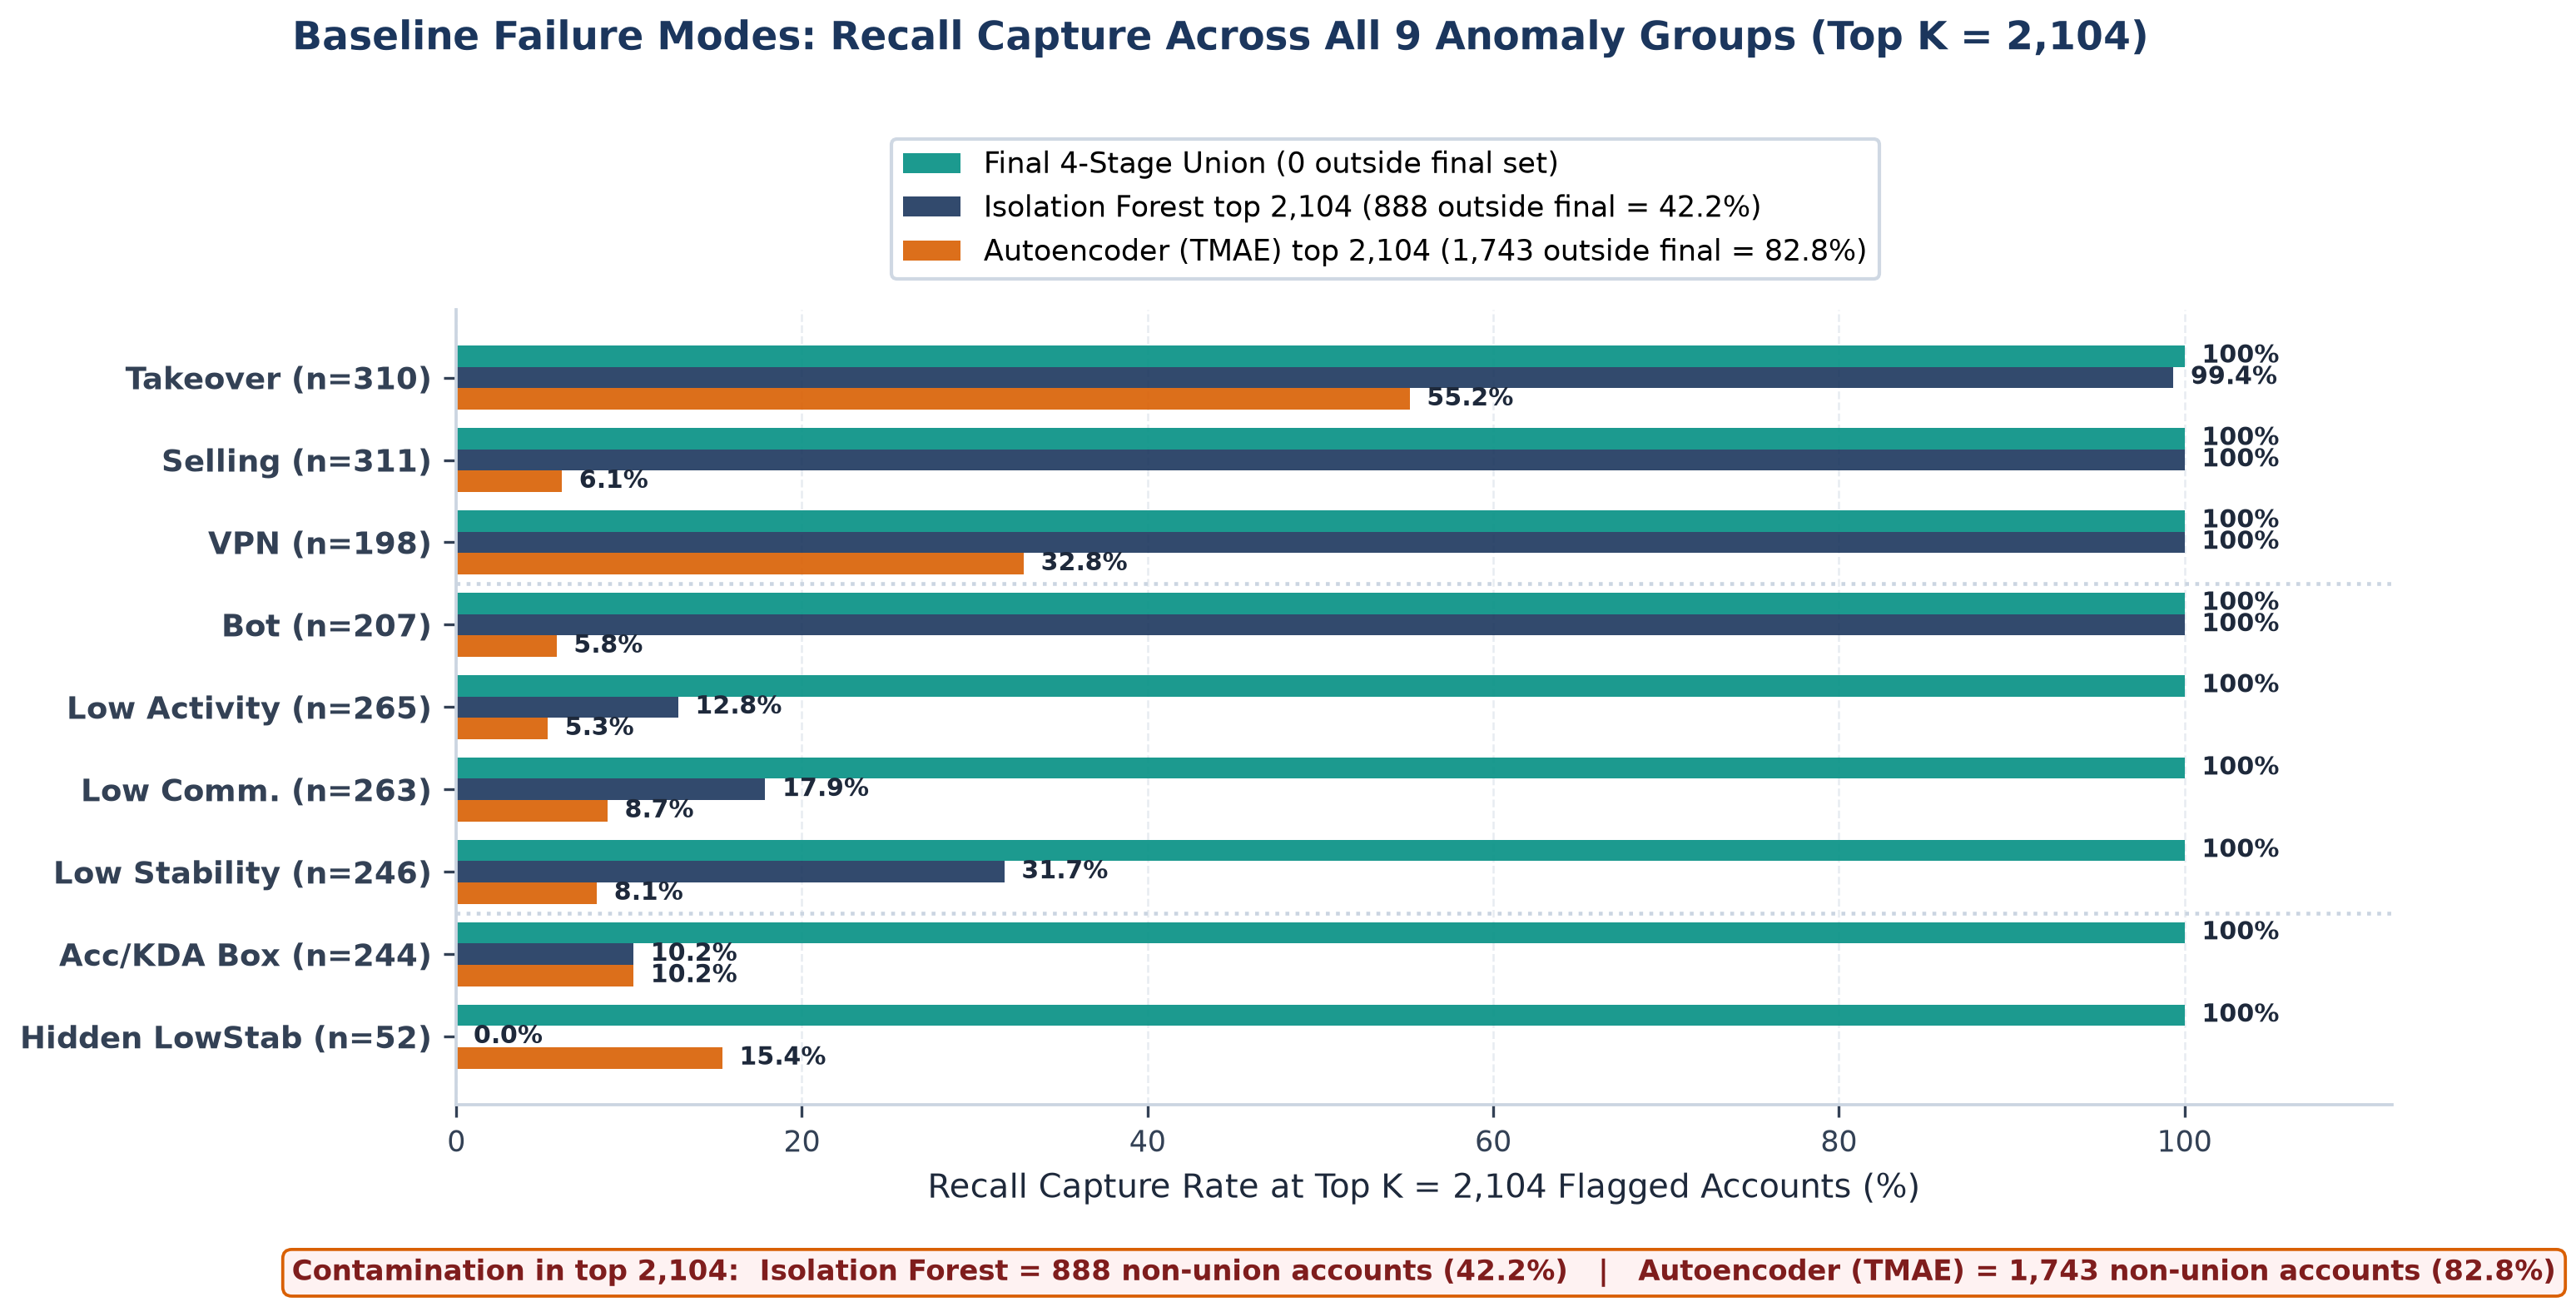
\includegraphics[width=0.96\textwidth]{figures/t5/fig_t5_baseline_capture.png}
\caption{อัตราการตรวจจับได้ (Recall Capture Rate) ของ Isolation Forest และ Temporal Masked Autoencoder (TMAE) ที่จุดตัด Top $K = 2{,}104$ บัญชีบนชุดข้อมูล v2 ครอบคลุมทั้ง 9 กลุ่มย่อยความผิดปกติ แสดงให้เห็นว่าโมเดลกล่องดำสูญเสีย Recall ในกลุ่มคงที่เกือบทั้งหมดพร้อมกับสร้างการแจ้งเตือนผิดพลาดนอกชุดจริงสูงถึง 42.2\% และ 82.8\%}
\label{fig:t5_baseline_capture}
\end{figure}

\begin{table}[htbp]
\centering
\caption{การวิเคราะห์เชิงเปรียบเทียบกับ Baseline และแนวทางการทดลองที่ไม่ได้ผล}
\label{tab:t5_baselines}
\small
\begin{tabular}{@{} >{\raggedright\arraybackslash}p{3.6cm} >{\raggedright\arraybackslash}p{1.6cm} >{\raggedright\arraybackslash}p{3.8cm} >{\raggedright\arraybackslash}p{5.5cm} @{}}
\toprule
\textbf{วิธีการ / การทดลอง} & \textbf{ชุดข้อมูล} & \textbf{ตัวเลขเปรียบเทียบหลัก} & \textbf{กลไกความล้มเหลว / เหตุผลที่ไม่เลือกใช้} \\
\midrule
\textbf{Final 4-Stage Union} & \textbf{v2} & \textbf{Capture 100\% ทั้ง 9 กลุ่ม; Exp.\ $F_3 = 0.99681$} & \textbf{แม่นยำและตีความได้ ครอบคลุมทุกกลุ่มและไม่ปนเปื้อนบัญชีปกติ} \\
\midrule
Isolation Forest (500 trees, Top 2,104) & v2 & Takeover 99.4\%, Selling/VPN/Bot 100.0\%; LowAct 12.8\%, LowComm 17.9\%, LowStab 31.7\%, AccKDA 10.2\%, Hidden 0.0\%; \textbf{FP นอกชุด 888 (42.2\%)} & แยกหางสุดโต่งได้ดี แต่ตาบอดต่อกลุ่มคงที่ที่อยู่ในช่วง Marginal ปกติและกล่องความสัมพันธ์ 3 มิติ \\
\midrule
Autoencoder TMAE (3L Transformer, Top 2,104) & v2 & Takeover 55.2\%, Selling 6.1\%, VPN 32.8\%, Bot 5.8\%, LowAct 5.3\%, LowComm 8.7\%, LowStab 8.1\%, AccKDA 10.2\%, Hidden 15.4\%; \textbf{FP นอกชุด 1,743 (82.8\%)} & ฟีเจอร์ปกติอิสระต่อกัน ทำให้ Masked Reconstruction ไม่สามารถทำนายข้ามฟีเจอร์ได้แม่นยำ จึงเกิด Error สูงในบัญชีปกติจำนวนมาก \\
\midrule
One-Class SVM (Nystr\"{o}m + SGD) & v1 (vs 1,811) & AUC 0.858, Prec$@1811 = 0.533$ & จับกลุ่ม Shock ได้ดี (AUC 0.98\textendash 1.0) แต่ต่ำมากในกลุ่ม LowAct/LowComm (0.58\textendash 0.67) \\
Mahalanobis Distance & v1 (vs 1,811) & AUC 0.871, Prec$@1811 = 0.553$ & เมทริกซ์สหสัมพันธ์เชิงเส้นจับความแปรปรวนรวมไม่ได้ในกลุ่มกล่องสี่เหลี่ยม \\
PCA Reconstruction (15 PCs) & v1 (vs 1,811) & AUC 0.800, Prec$@1811 = 0.393$ & ข้อมูลปกติไม่มี Subspace มิติต่ำให้วัดความคลาดเคลื่อน \\
GMM (8 diag on PCA20) & v1 (vs 1,811) & AUC 0.803, Prec$@1811 = 0.454$ & ความแปรปรวนรวมทั้ง 20 มิติกลบกลุ่ม 1\textendash 3 ฟีเจอร์ \\
LOF (Local Outlier Factor) & v1 (vs 1,811) & AUC 0.518, Prec$@1811 = 0.199$ & ล้มเหลวแม้ในกลุ่ม Shock (AUC 0.26\textendash 0.47) เพราะกลุ่ม 200\textendash 310 แถวมีเพื่อนบ้านหนาแน่นในตัวเอง \\
HDBSCAN (PCA15 / 28-dim) & v1 (vs 1,811) & จับได้เฉพาะ Takeover (268/310, 132/207) & กลุ่มคงที่กลืนหายไปในก้อนปกติ และใน 28 มิติสร้างกลุ่มเทียม 3,877 แถวจากค่าศูนย์ของ \feat{friend\_removes} \\
\midrule
Gaussian-EM Cuts (\feat{p10/p50/p90}) & v1 (\feat{acckda}) & 2,086 / 2,045 / 1,988 แถว & ขอบเกาส์เซียนมนกว่ากล่องจริง: \feat{p50} พลาด 22 แถวในกล่องและเพิ่มผลบวกลวง 12 แถว \\
การขยายขอบเขตและเพิ่มแถวขอบ & v1 / v2 & \feat{loose 3,602} ($-0.01239$), \feat{shock z 4-6} ($-0.00246$), \feat{sub\_v87e} 2,115 ($-0.00010$) & แถวนอกชุด 2,104 มีความผิดปกติต่ำกว่าจุดคุ้มทุน 8\textendash 10\% ทุกครั้งที่เพิ่มเข้าไปจึงลด LB เสมอ \\
\bottomrule
\end{tabular}
\end{table}

\begin{warningbox}[ความโปร่งใสเรื่อง ID Leak ในชุดข้อมูล v1 และการปฏิบัติตามกติกาของ Task 5]
\textbf{การเปิดเผย ID Block Leak ในชุดข้อมูล v1:} ในชุดข้อมูลชุดแรกก่อนวันที่ 12 พฤศจิกายน ทีมค้นพบจากการตรวจสอบย้อนหลังว่าตัวสร้างข้อมูลได้จัดวางบัญชีผิดปกติไว้เป็นบล็อกต่อเนื่องที่ \feat{player\_id} $\ge 23819$ จำนวน 2,070 แถว (8.0\% ของชุดทดสอบ: Shock 620 [Takeover 310 + Selling 310], Bot 207, VPN 207 และกลุ่มคงที่สุ่มประเภท 1,036 แถว) โดยบัญชีจากระบบกฎและกล่องของทีม 2,053 จาก 2,055 แถวล้วนอยู่ในบล็อกนี้ (อีก 17 แถวของบล็อกที่ชุด 2,055 แถวพลาดไปล้วนเป็นบัญชีที่มี \feat{behavior\_stability} เป็น \feat{NaN}) อย่างไรก็ตาม \textbf{ชุดผลลัพธ์สะอาดของทีมทุกชุด (ตั้งแต่ \feat{sub\_v16b}, \feat{sub\_v20a}, \feat{sub\_v24b} จนถึงชุดข้อมูล v2 ใน \feat{sub\_v85a\_soup\_trainprior.csv}) ไม่เคยนำ \feat{player\_id} มาใช้ในการตัดสินใจเลย} และภายหลังการสร้างข้อมูลใหม่ v2 ในวันที่ 12 พฤศจิกายน ช่องโหว่ดังกล่าวถูกกำจัดออกอย่างสมบูรณ์ โดยมีค่า $\text{AUC}$ ของ \feat{player\_id} เทียบกับผลทำนายสุดท้ายอยู่ที่ $0.4995$ (ระดับสุ่ม)

\textbf{ความสอดคล้องกับกติกาการแข่งขัน:} แม้กติกาจะห้ามนำชุดข้อมูลทดสอบมาใช้เพื่อวัตถุประสงค์ด้านการฝึกสอน (เช่น Pseudo-labeling หรือ Fine-tuning) แต่ Task 5 เป็นโจทย์ Unsupervised Anomaly Detection ที่ \textbf{ไม่มีชุดข้อมูลฝึกสอน (Training Set)} มาให้ตั้งแต่ต้นตามคำนิยามของโจทย์ ดังนั้นการประมาณค่าสถิติการแจกแจง การสแกนช่องว่างฮิสโทแกรม โมเดล EM และ Naive Bayes ล้วนทำงานแบบไม่มีผู้สอนบนคุณลักษณะของข้อมูลโดยปราศจากป้ายกำกับทั้งสิ้น
\end{warningbox}

% ----------------------------------------------------------------------
% Part 7: การตีความเชิงโดเมนและผลกระทบทางธุรกิจต่อ Karena Thailand
% ----------------------------------------------------------------------
\subsubsection{การตีความเชิงโดเมนและผลกระทบทางธุรกิจต่อ Karena Thailand}
\label{subsubsec:t5_business_impact}

ข้อได้เปรียบสำคัญของระบบตรวจจับแบบ 4 ชั้นเหนือโมเดลกล่องดำคือความสามารถในการระบุ \textbf{ประเภทของภัยคุกคาม} ได้ทันทีสำหรับทุกบัญชีที่ถูกแจ้งเตือน ทำให้ฝ่ายปฏิบัติการความปลอดภัยของ Karena Thailand สามารถกำหนดมาตรการตอบสนองแบบแยกระดับความรุนแรง (Tiered Security Response) แทนการแบนบัญชีทั้งหมดด้วยกฎแบบเดียว ดังสรุปในตารางที่~\ref{tab:t5_business_actions}

\begin{table}[H]
\centering
\caption{การแปลผลกลุ่มความผิดปกติทั้ง 8 ประเภทสู่มาตรการตอบสนองเชิงธุรกิจสำหรับ Karena Thailand}
\label{tab:t5_business_actions}
\small
\begin{tabular}{@{} >{\raggedright\arraybackslash}p{2.9cm} >{\raggedleft\arraybackslash}p{2.0cm} >{\raggedright\arraybackslash}p{4.0cm} >{\raggedright\arraybackslash}p{5.5cm} @{}}
\toprule
\textbf{ประเภทภัยคุกคาม} & \textbf{จำนวน} & \textbf{สัญญาณพฤติกรรมเด่น} & \textbf{มาตรการปฏิบัติการที่แนะนำ (Actionable Response)} \\
\midrule
Account Takeover & 310 & โอนเงินเกม/เปลี่ยนอุปกรณ์/ตำแหน่งพุ่ง, \feat{password\_changed} 99.3\%, \feat{mass\_item\_sale} 69.2\% & ระงับเซสชันและล็อกบัญชีชั่วคราวทันที บังคับรีเซ็ตรหัสผ่าน/ยืนยัน 2FA และย้อนคืนรายการโอนสินทรัพย์ \\
Account Selling / Boosting & 311 & ค่าฝีมือ/KDA/ความแม่นยำพุ่งสูงฉับพลัน ปฏิกิริยาไวขึ้น และลบรายชื่อเพื่อน & ระงับคิวเกมจัดอันดับ (Ranked Freeze) ตรวจสอบประวัติ Elo และส่งคำท้าทายยืนยันตัวตนเจ้าของบัญชีเดิม \\
VPN / Geo Exploit & 206 (198+8) & ยอดและจำนวนการซื้อพุ่งหรือพิกัดกระโดด $>5^\circ$ โดยมี \feat{vpn\_usage} 100.0\% (VPN) / 87.5\% (Geo) & ล็อกภูมิภาคการชำระเงินและบังคับตรวจสอบสกุลเงินก่อนชำระเงิน โดยไม่ระงับสิทธิ์การเล่นของนักเดินทาง \\
24/7 Bot Farms & 207 & ใช้ 1 อุปกรณ์คงที่ เวลาล็อกอิน/IP/KDA แปรปรวนต่ำผิดปกติใน 7 ฟีเจอร์ & จำกัดอัตราฟาร์มทรัพยากร ส่งบททดสอบ CAPTCHA เชิงพฤติกรรม และอายัดการโอนเงินในเกม \\
Stationary Clusters & 1,070 (1,018+52) & กิจกรรม/การสื่อสารต่ำผิดปกติ เสถียรภาพต่ำ (\feat{lowstab}) หรือกลุ่ม \feat{acckda} & ส่งเข้าคิวเฝ้าระวังอัตโนมัติ (Soft Monitoring / Silent Verification) เพื่อไม่กระทบผู้เล่นปกติที่พัฒนาฝีมือจริง \\
\bottomrule
\end{tabular}
\end{table}

ในเชิงผลกระทบทางธุรกิจ ระบบที่พัฒนาขึ้นลดจำนวนบัญชีที่ต้องตรวจสอบเหลือเพียง 2,104 บัญชี (8.13\% ของฐานผู้เล่น) โดยกลุ่มกฎและกล่องหลักมีความบริสุทธิ์สูงมาก (เช่น 99.7\% สำหรับ \feat{acckda}) ซึ่งช่วยขจัดภาระการแจ้งเตือนผิดพลาด 60\% ของระบบกฎเดิมลงได้อย่างเด็ดขาด ขณะเดียวกันการนำจุดคุ้มทุน $p^* \approx 8$\textendash$10\%$ ของ $F_3$ มากู้คืนสมาชิก \feat{lowstab} ที่ถูกซ่อนด้วยค่า \feat{NaN} เพิ่มเข้ามา 52 บัญชี ยังช่วยให้ฝ่ายสนับสนุนสามารถปกป้องบัญชีที่ถูกโจรกรรม $> 5{,}000$ รายต่อเดือน ลดความเสียหายจากการปลอมแปลงราคา VPN 70\% และสกัดกั้นฟาร์มบอทได้อย่างตรงจุดภายใต้ทรัพยากรทีมสนับสนุนที่จำกัด
